\section{Aproximación cuasiestática}

El \textit{límite cuasiestático} consiste en considerar el tamaño de la partícula a estudiar mucho menor que la longitud de onda de la luz incidente. En el caso de un elipsoide caracterizado por una función dieléctrica $\epsilon_1$, de semieje mayor $a$, se debe de considerar a este último mucho menor que la longitud de onda de la luz incidente $\lambda$. Esta aproximación garantiza que el elipsoide esté sujeto a un campo eléctrico de la misma intensidad y dirección. \cite{Miguel}\\


En distancias mucho mayores que el tamaño de una partícula, es posible aproximar a esta como un \textit{dipolo eléctrico puntual}, por lo cual, es conveniente estudiar el potencial y campo eléctrico que produce.\\

Un dipolo eléctrico consiste en dos cargas puntuales $q$ y $-q$ separadas a una distancia $d$ (ver Fig.\ref{dipolo_elec}), con momento dipolar $\Vec{p}=p\hat{e}_z$ donde $p=qd$. Si las cargas se encuentran embebidas en un medio homogéneo e infinito con función dieléctrica $\epsilon_m$, entonces el potencial $\phi$ del dipolo en cualquier punto $P$ es \cite{Bohren,Griffiths}
\begin{equation}
    \phi=\frac{q}{4\pi\epsilon_m}\left(\frac{1}{r_+}-\frac{1}{r_{-}}\right),    
\end{equation}
donde, usando la ley de cosenos y considerando que $\cos\theta=\frac{\Vec{r}\cdot\hat{e}_z}{r}$, se tiene que 
\begin{align*}
    r_{\pm}^2&=r^2+\left(\frac{d}{2}\right)^2 \mp rd\cos\theta=r^2\left(1+\left(\frac{d}{2r}\right)^2\mp \frac{d\cos\theta}{r}\right)=r^2\left(1+\left(\frac{d}{2r}\right)^2\mp \frac{\Vec{r}\cdot\hat{e}_z}{r^2}d\right),
\end{align*}
o bien,
\begin{equation*}
  \frac{1}{r_{\pm}}=\frac{1}{r}\left(1+\left(\frac{d}{2r}\right)^2\mp \frac{\Vec{r}\cdot\hat{e}_z}{r^2}d\right)^{-1/2}.  
\end{equation*}
\begin{figure}[h!]
    \centering
    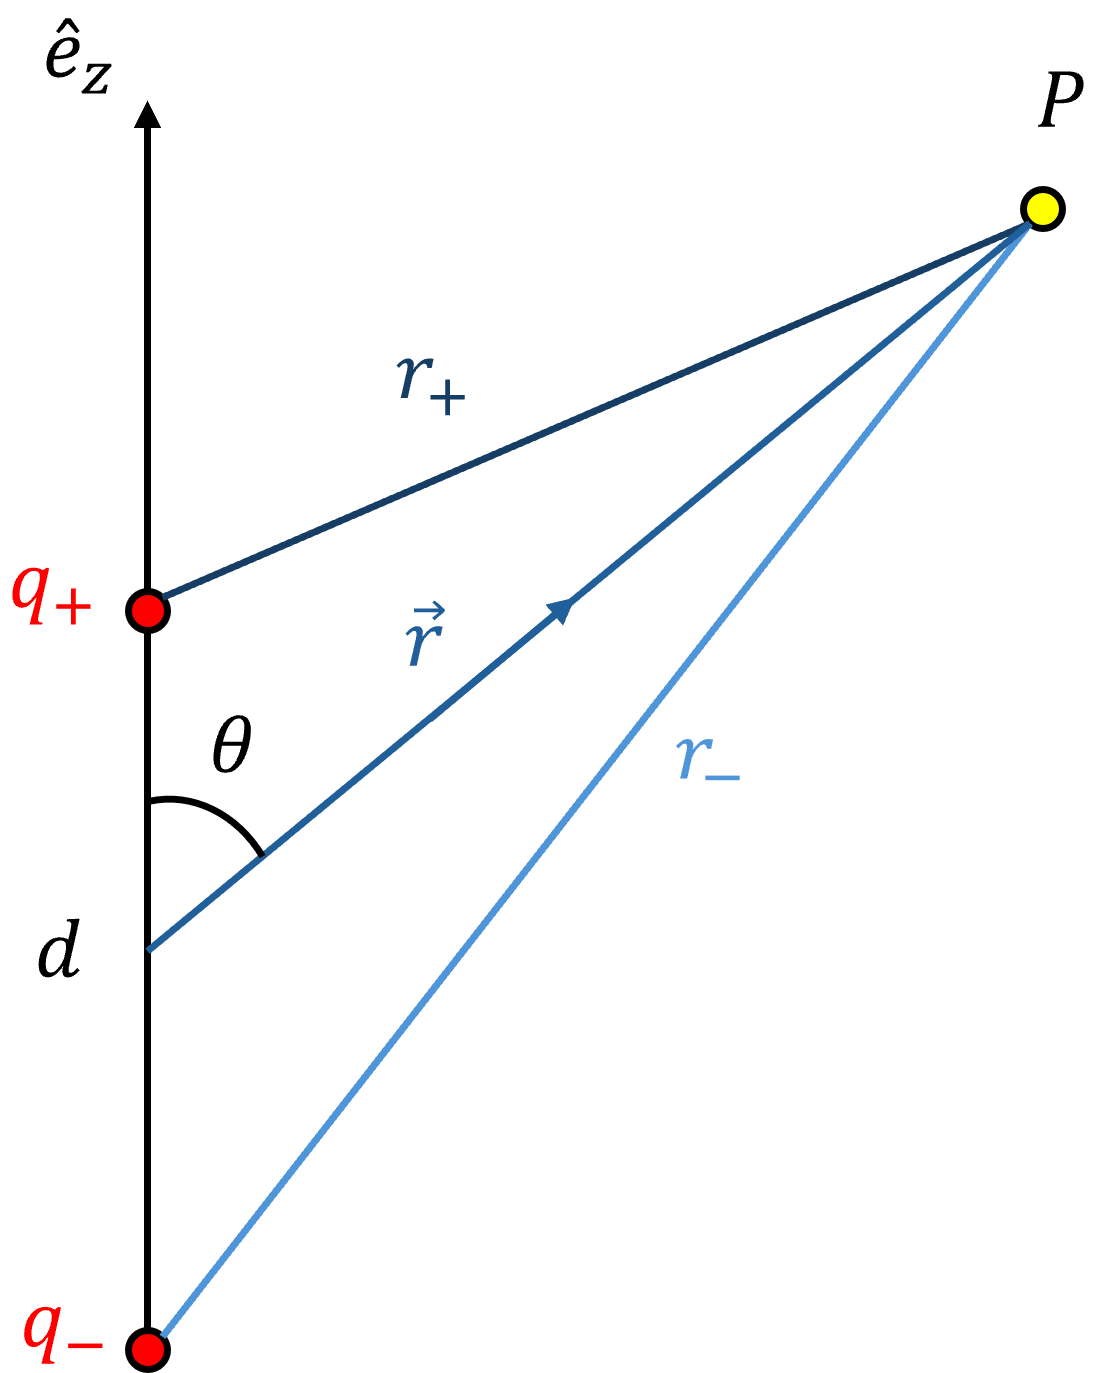
\includegraphics[width=5cm1]{../../../../Pictures/servicio social/dipolo.png} 
    \caption{Dipolo eléctrico.}
    \label{dipolo_elec}
\end{figure}
Como la región de interés es para $r\gg d$, entonces el segundo término tiende a 0 y se tiene que
\begin{equation*}
    \frac{1}{r_{\pm}}\approx\frac{1}{r}\left(1\mp \frac{\Vec{r}\cdot\hat{e}_z}{r^2}d\right)^{-1/2},
\end{equation*}
luego, usando la expansión binomial a primer orden de $(1\mp x)^n=1+nx$,  se tendrá que
\begin{equation*}
    \frac{1}{r_{\pm}}\approx\frac{1}{r}\left(1\pm \frac{\Vec{r}\cdot\hat{e}_z}{2r^2}d\right).
\end{equation*}
De esta forma,
\begin{equation}
    \frac{1}{r_+}-\frac{1}{r_{-}}=\frac{1}{r}\left(1+ \frac{\Vec{r}\cdot\hat{e}_z}{2r^2}d-1+ \frac{\Vec{r}\cdot\hat{e}_z}{2r^2}d\right)=\frac{1}{r}\left( \frac{\Vec{r}\cdot\hat{e}_z}{r^2}d\right)=\frac{\Vec{r}\cdot\hat{e}_z}{r^3}d.    
\end{equation}

Si $d$ se aproxima a cero de tal forma que $qd$ permanezca constante, se obtiene el potencial para un dipolo puntual
\begin{equation}
\phi=\frac{p}{4\pi\epsilon_m}\left(\frac{\Vec{r}\cdot\hat{e}_z}{r^3}\right)=\frac{\Vec{p}\cdot\Vec{r}}{4\pi\epsilon_m r^3}=\frac{p\cos\theta}{4\pi\epsilon_m r^2}.
\label{pot_dipolo}
\end{equation}

Considerando un sistema de cargas y corrientes variando con el tiempo, se puede hacer una expansión en series de Fourier de la dependencia del tiempo y manejar cada componente de Fourier por separado. De esta forma, no se pierde generalidad de considerar a los potenciales y campos de un sistema localizado de cargas y corrientes variando en el tiempo \cite{Jackson}
\begin{align*}
    \rho(\Vec{r},t)&=\rho(\Vec{r})e^{-i\omega t},\\
    \Vec{J}(\Vec{r},t)&=\Vec{J}(\Vec{r})e^{-i\omega t},
\end{align*}
considerando que el significado físico lo posee la parte real. Las fuentes estarán consideradas localizadas en el espacio vacío.\\

De acuerdo con la norma de Lorenz se tiene que la solución para el potencial vectorial $\Vec{A}(\Vec{r},t)$ es \cite{Jackson}
\begin{align}
  \Vec{A}(\Vec{r},t)&=\frac{\mu_0}{4\pi}\int d^3r'\int dt'\frac{\Vec{J}(\Vec{r'},t')}{|\Vec{r}-\Vec{r'}|}\delta\left(t'-\left(t-\frac{|\Vec{r}-\Vec{r'}|}{c}\right)\right)\nonumber\\
  &=\frac{\mu_0}{4\pi}\int d^3r'\frac{\Vec{J}(\Vec{r'})e^{-i\omega \left(t-\frac{|\Vec{r}-\Vec{r'}|}{c}\right)}}{|\Vec{r}-\Vec{r'}|}=\frac{\mu_0}{4\pi}\int d^3r'\frac{\Vec{J}(\Vec{r'})e^{i\omega \frac{|\Vec{r}-\Vec{r'}|}{c}}}{|\Vec{r}-\Vec{r'}|}e^{-i\omega t},
\end{align}
donde la función Delta de Dirac asegura el comportamiento causal de los campos electromagnéticos.\\

Sea $k=\omega/c$ y omitiendo la dependencia temporal
\begin{equation}
    \Vec{A}(\Vec{r},t)=\frac{\mu_0}{4\pi}\int \Vec{J}(\Vec{r'})\frac{e^{ik|\Vec{r}-\Vec{r'}|}}{|\Vec{r}-\Vec{r'}|} d^3r',
    \label{pot_vectorial}
\end{equation} 

Considerando un tiempo $t>t-\frac{|\Vec{r}-\Vec{r}'|}{c}$ y el carácter sinusoidal dependiente del tiempo se tiene que

\begin{equation}
\Vec{A}(\Vec{r})=\frac{\mu_0}{4\pi}\int \Vec{J}(\Vec{r}')\frac{e^{ik}}{|\Vec{r}-\Vec{r}'|} d^3r'.
\end{equation}
Luego, dadas las ecuaciones de Maxwell
\begin{align}
    \nabla\cdot\Vec{E}&=0,\\
    \nabla\cdot\Vec{H}&=0,\\
    \nabla\times\Vec{E}&=i\omega\mu\Vec{H},\\
    \nabla\times\Vec{H}&=-i\omega\epsilon\Vec{E},\\
\end{align}
y como $\Vec{B}=\nabla\times\Vec{A}, \Vec{H}=\frac{\Vec{B}}{\mu_0}-\Vec{M}=\frac{\Vec{B}}{\mu_0}$, entonces 
\begin{equation}
    \Vec{H}=\frac{1}{\mu_0}\nabla\times\Vec{A}\hspace{0.5cm}\mbox{y}\hspace{0.5cm}    \Vec{E}=\frac{i}{\omega\epsilon}\nabla\times\Vec{H}.
\end{equation}
Si las dimensiones de la fuente son del orden $d$ y la longitud de onda es $\lambda=2\pi c/\omega$, y $d\ll\lambda$, entonces hay tres regiones de interés \cite{Jackson}
\begin{itemize}
    \item La región cercana (estática): \hspace{2.4cm}$d\ll r\ll\lambda$
    \item La región intermedia (inducción):\hspace{1.7cm}$d\ll r\sim \lambda$
    \item La región lejana (de radiación):\hspace{2cm}$d\ll \lambda\ll r$
\end{itemize}
En la región de campo cercano los campos son como los campos estáticos con componentes radiales. En la región de campo lejano, los campos son transversales al vector radial y decaen como $r^{-1}$. 
Para la región de campo cercano donde $r\ll\lambda$ (o $kr\ll 1$) la exponencial del potencial vectorial puede ser reemplazada por 1 y con ello encontramos la expresión conocida de este.
En la región de campo lejano ($kr\gg 1$) dado que la exponencial oscila rápidamente, determina el comportamiento del potencial vectorial. En esta región es suficiente aproximar:
\begin{equation}
    |\Vec{r}-\Vec{r'}|\simeq r-\hat{e}_r\cdot\Vec{r'},    
\end{equation}
con $\hat{e}_r$ un vector unitario en la dirección de $\Vec{r}$. Más aún, considerando la región de campo lejano, si sólo se consideran los términos que decaen como $r^{-1}$, la distancia inversa en Ec.( \ref{pot_vectorial}) puede ser reemplazada por $r$. Entonces, el potencial vectorial es
\begin{equation*}
    \lim_{kr\rightarrow\infty}\Vec{A}(\Vec{r})=\frac{\mu_0}{4\pi}\frac{e^{ikr}}{r}\int \Vec{J}(\Vec{r'})e^{-ik\hat{e}_r\cdot\Vec{r'}}d^3r',    
\end{equation*}
donde además se puede expandir en potencias de $k$:
\begin{equation*}
    \lim_{kr\rightarrow\infty}\Vec{A}(\Vec{r})=\frac{\mu_0}{4\pi}\frac{e^{ikr}}{r}\sum_n\frac{(-ik)^n}{n!}\int \Vec{J}(\Vec{r'})(\hat{e}_r\cdot\Vec{r'})^n d^3r'.    
\end{equation*}
Si sólo se conserva el primer término de la expresión anterior
\begin{equation}
    \Vec{A}(\Vec{r})=\frac{\mu_0}{4\pi}\frac{e^{ikr}}{r}\int \Vec{J}(\Vec{r'}) d^3r',    
\end{equation}
integrando por partes,
$$\int\Vec{J}d^3r'=-\int \Vec{r'}(\nabla'\cdot\Vec{J})d^3r'=-i\omega\int \Vec{r'}\rho(\Vec{r'})d^3r',$$
de donde se usa la ecuación de continuidad
\begin{equation}
    \nabla\cdot\Vec{J}=-\frac{\partial\rho}{\partial t}=i\omega\rho(\Vec{r}).    
\end{equation}
Entonces, 
\begin{equation}
    \Vec{A}(\Vec{r})=-\frac{i\omega\mu_0}{4\pi}\frac{e^{ikr}}{r}\int \Vec{r'}\rho(\Vec{r'})d^3r'=-\frac{i\omega\mu_0}{4\pi}\frac{e^{ikr}}{r}\Vec{p} ,   
\end{equation}
con $\Vec{p}$ el momento dipolar eléctrico.
De esto se sigue que los campos de un dipolo eléctrico son (ver \textit{Apéndice})
\begin{align}
    \Vec{H}&=\frac{1}{\mu_0}\nabla\times\Vec{A}=\frac{ck^2}{4\pi}(\hat{e}_r\times\Vec{p})\frac{e^{ikr}}{r}\left(1-\frac{1}{ikr}\right),\\
    \Vec{E}&=\frac{i}{\omega\epsilon}\nabla\times\Vec{H}=\frac{1}{4\pi\epsilon_0}\left\{k^2(\hat{e}_r\times\Vec{p})\times\hat{e}_r\frac{e^{ikr}}{r}+[3\hat{e}_r(\hat{e}_r\cdot\Vec{p})-\Vec{p}]\left(\frac{1}{r^3}-\frac{ik}{r^2}\right)e^{ikr}\right\}.
\end{align}
Obsérvese que el campo $\Vec{H}$ es transversal al vector radial para cualquier distancia, mientras el campo eléctrico tiene componentes paralelas y perpendiculares a $\hat{e}_r$.\\

\noindent En la zona de radiación cuando $kr\gg 1$ se tiene que
\begin{align}
    \Vec{H}&=\frac{ck^2}{4\pi}(\hat{e}_r\times\Vec{p})\frac{e^{ikr}}{r}\\
    \Vec{E}&=\sqrt{\frac{\mu_0}{\epsilon_0}}\Vec{H}\times\hat{e}_r=\frac{ck^2}{4\pi}(\hat{e}_r\times\Vec{p})\times\Vec{e}_r\frac{e^{ikr}}{r}=\frac{e^{ikr}}{-ikr}\frac{ik^3}{4\pi\epsilon_m}\hat{e}_r\times(\hat{e}_r\times\Vec{p}).
\end{align}
Si el momento dipolar oscila a la frecuencia del campo incidente, entonces el dipolo radía campo electromagnético, es decir, esparce un campo eléctrico $\Vec{E_{scat}}$ dado por
\begin{equation}
    \Vec{E}_{scat}=\frac{e^{ikr}}{-ikr}\frac{ik^3}{4\pi\epsilon_m}\hat{e}_r\times(\hat{e}_r\times p)  ,  
\end{equation}
donde el factor de dependencia temporal $e^{i\omega t}$ se ha omitido. Sustituyendo el momento dipolar de un dipolo puntual $\Vec{p}=\epsilon_m \alpha E_0 e^{-i\omega t}\hat{e}_x$, se tiene que podemos reescribir al campo esparcido como
$$\Vec{E}_{scat}=\frac{e^{ikr}}{-ikr}\frac{ik^3}{4\pi\epsilon_m}\left(\epsilon_m \alpha E_0 \right)\hat{e}_r\times(\hat{e}_r\times \hat{e}_x)=\frac{e^{ik(r-z)}}{-ikr}\frac{ik^3}{4\pi}\left( \alpha E_0 e^{ikz}\right)\hat{e}_r\times(\hat{e}_r\times \hat{e}_x)=\frac{e^{ik(r-z)}}{-ikr}\Vec{X}E,$$
donde $E=E_0 e^{ikz}$ y $\Vec{X}=\frac{ik^3}{4\pi}\alpha \hat{e}_r\times(\hat{e}_r\times \hat{e}_x)$ es
el vector de amplitud de esparcimiento. Más aún, $\hat{e}_r\times(\hat{e}_r\times \hat{e}_x)=-\cos\theta\cos\phi \hat{e}_{\theta}+\sin\phi \hat{e}_{\phi}$. \\

Dado el coeficiente de extinción \cite{Bohren}
\begin{equation}
    C_{ext}=\frac{W_{ext}}{I_i}=\frac{4\pi}{k^2} \mbox{Re}\{(\Vec{X}\cdot\hat{e}_x)_{\theta=0}\}    
\end{equation}
como
\begin{equation}
    \Vec{X}\cdot\hat{e}_x=\frac{ik^3}{4\pi}\alpha \hat{e}_r\times(\hat{e}_r\times \hat{e}_x)\cdot\hat{e}_x=\frac{ik^3}{4\pi}\alpha\left(\hat{e}_r(\hat{e}_r\cdot \hat{e}_x)-\hat{e}_x(\hat{e}_r\cdot \hat{e}_r)\right)\cdot\hat{e}_x=\frac{ik^3}{4\pi}\alpha(\sin^2\theta\cos^2\phi-1),    
\end{equation}
entonces, 
\begin{equation}
    C_{ext}=k \mbox{Re}\left[\left(i\alpha(\sin^2\theta\cos^2\phi-1)\right)_{\theta=0}\right]=k\:\mbox{Re}\left[-i\alpha\right],
\end{equation}
pero la polarizabilidad es compleja $\alpha=\alpha_1+i\alpha_2$, por lo que $-i\alpha=\alpha_2-i\alpha_1$; de forma que la parte real de $-i\alpha$ es igual a la parte imaginaria de $\alpha$, por lo que se sigue que
\begin{equation}
    C_{ext}=k\: \mbox{Im}[\alpha].    
\end{equation}
Asimismo, el coeficiente de esparcimiento está descrito por \cite{Bohren}
\begin{align}
    C_{scat}&=\int_{0}^{2\pi}\int_0^{\pi}\frac{|\Vec{X}|^2}{k^2}\sin\theta d\theta d\phi\nonumber\\
    &=\frac{(\alpha\cdot\alpha^*)k^4}{(4\pi)^2}\int_0^{2\pi}\int_0^{\pi}(\sin^2\theta\cos^2\phi+1)\sin\theta d\theta d\phi\nonumber\\
    &=\frac{|\alpha|^2k^4}{(4\pi)^2}\frac{8\pi^2}{3}=\frac{|\alpha|^2k^4}{6\pi},
\end{align}
y se tiene que \cite{Bohren}
\begin{equation}
    C_{abs}=C_{ext}-C_{scat}.    
\end{equation}
